\documentclass[journal]{vgtc}                % final (journal style)
%\documentclass[review,journal]{vgtc}         % review (journal style)
%\documentclass[widereview]{vgtc}             % wide-spaced review
%\documentclass[preprint,journal]{vgtc}       % preprint (journal style)
%\documentclass[electronic,journal]{vgtc}     % electronic version, journal

%% Uncomment one of the lines above depending on where your paper is
%% in the conference process. ``review'' and ``widereview'' are for review
%% submission, ``preprint'' is for pre-publication, and the final version
%% doesn't use a specific qualifier. Further, ``electronic'' includes
%% hyperreferences for more convenient online viewing.

%% Please use one of the ``review'' options in combination with the
%% assigned online id (see below) ONLY if your paper uses a double blind
%% review process. Some conferences, like IEEE Vis and InfoVis, have NOT
%% in the past.

%% Please note that the use of figures other than the optional teaser is not permitted on the first page
%% of the journal version.  Figures should begin on the second page and be
%% in CMYK or Grey scale format, otherwise, colour shifting may occur
%% during the printing process.  Papers submitted with figures other than the optional teaser on the
%% first page will be refused.

%% These three lines bring in essential packages: ``mathptmx'' for Type 1
%% typefaces, ``graphicx'' for inclusion of EPS figures. and ``times''
%% for proper handling of the times font family.

\usepackage{mathptmx}
\usepackage{graphicx}
\usepackage{times,amsfonts,amssymb,amsthm}
\usepackage{times}
\usepackage{amsfonts}
\usepackage{amsthm}
\usepackage{amsmath}
\usepackage{subcaption}
\usepackage{comment}

\theoremstyle{definition}
\newtheorem{defn}{Definition} % definition numbers are dependent on theorem numbers
\newtheorem{theorem}{Theorem} % definition numbers are dependent on theorem numbers

%% commands
\newcommand{\cP}{\mathcal{P}}
\newcommand{\R}{\mathbb{R}}
\newcommand{\cM}{\mathcal{M}}
\newcommand{\primoz}[1]{\textcolor{red}{#1}}
\newcommand{\lstopar}[1]{\textcolor{blue}{#1}}

\newcommand{\argmin}{\operatornamewithlimits{argmin}}
\DeclareMathOperator{\Ima}{Im}

\graphicspath{{img/}}

%% We encourage the use of mathptmx for consistent usage of times font
%% throughout the proceedings. However, if you encounter conflicts
%% with other math-related packages, you may want to disable it.

%% This turns references into clickable hyperlinks.
\usepackage[bookmarks,backref=true,linkcolor=black]{hyperref} %,colorlinks
\hypersetup{
  pdfauthor = {},
  pdftitle = {},
  pdfsubject = {},
  pdfkeywords = {},
  colorlinks=true,
  linkcolor= black,
  citecolor= black,
  pageanchor=true,
  urlcolor = black,
  plainpages = false,
  linktocpage
}

%% If you are submitting a paper to a conference for review with a double
%% blind reviewing process, please replace the value ``0'' below with your
%% OnlineID. Otherwise, you may safely leave it at ``0''.
\onlineid{0}

%% declare the category of your paper, only shown in review mode
\vgtccategory{Research}

%% allow for this line if you want the electronic option to work properly
\vgtcinsertpkg

%% In preprint mode you may define your own headline.
%\preprinttext{To appear in an IEEE VGTC sponsored conference.}

%% Paper title.

\title{A Multi-Scale Methodology for Explaining Data Streams}

%% This is how authors are specified in the journal style

%% indicate IEEE Member or Student Member in form indicated below
\author{Luka Stopar and Primoz Skraba}
\authorfooter{
%% insert punctuation at end of each item
\item
Luka Stopar is with Jozef Stefan Institute. E-mail: luka.stopar@ijs.si.
\item
Primoz Skraba is with Jozef Stefan Institute. E-mail: primoz.skraba@ijs.si.
}

%other entries to be set up for journal
\shortauthortitle{Stopar \MakeLowercase{\textit{et al.}}: A Multi-Level Methodology for Explaining Data Streams}
%\shortauthortitle{Firstauthor \MakeLowercase{\textit{et al.}}: Paper Title}

%% Abstract section.
\abstract{
	This paper presents a novel multi-scale methodology for modeling, visualization and summarization of a collection
	of continuously time-varying data streams. The proposed methodology represents such a collection in qualitative 
	manner using a novel hierarchical framework by partitioning and aggregating the data streams using unsupervised data mining
	methods and constructing a Markovian transition model, capturing the dynamics of the data. The resulting model
	provides a visual summary and allows users to explore the data on several scales.  We validate our methodology on
	three real-world datasets.
} % end of abstract

%% Keywords that describe your work. Will show as 'Index Terms' in journal
%% please capitalize first letter and insert punctuation after last keyword
\keywords{Visualization, Data Streams, Multi-Scale, Summarization, Markov Chains, Exploratory Data Mining, \lstopar{do these need to be in some index?}}

%% ACM Computing Classification System (CCS). 
%% See <http://www.acm.org/class/1998/> for details.
%% The ``\CCScat'' command takes four arguments.

\CCScatlist{ % not used in journal version
 \CCScat{K.6.1}{Management of Computing and Information Systems}%
{Project and People Management}{Life Cycle};
 \CCScat{K.7.m}{The Computing Profession}{Miscellaneous}{Ethics}
}



% Uncomment below to include a teaser figure.
\teaser{
	\label{fig:teaser}
 	\centering
 	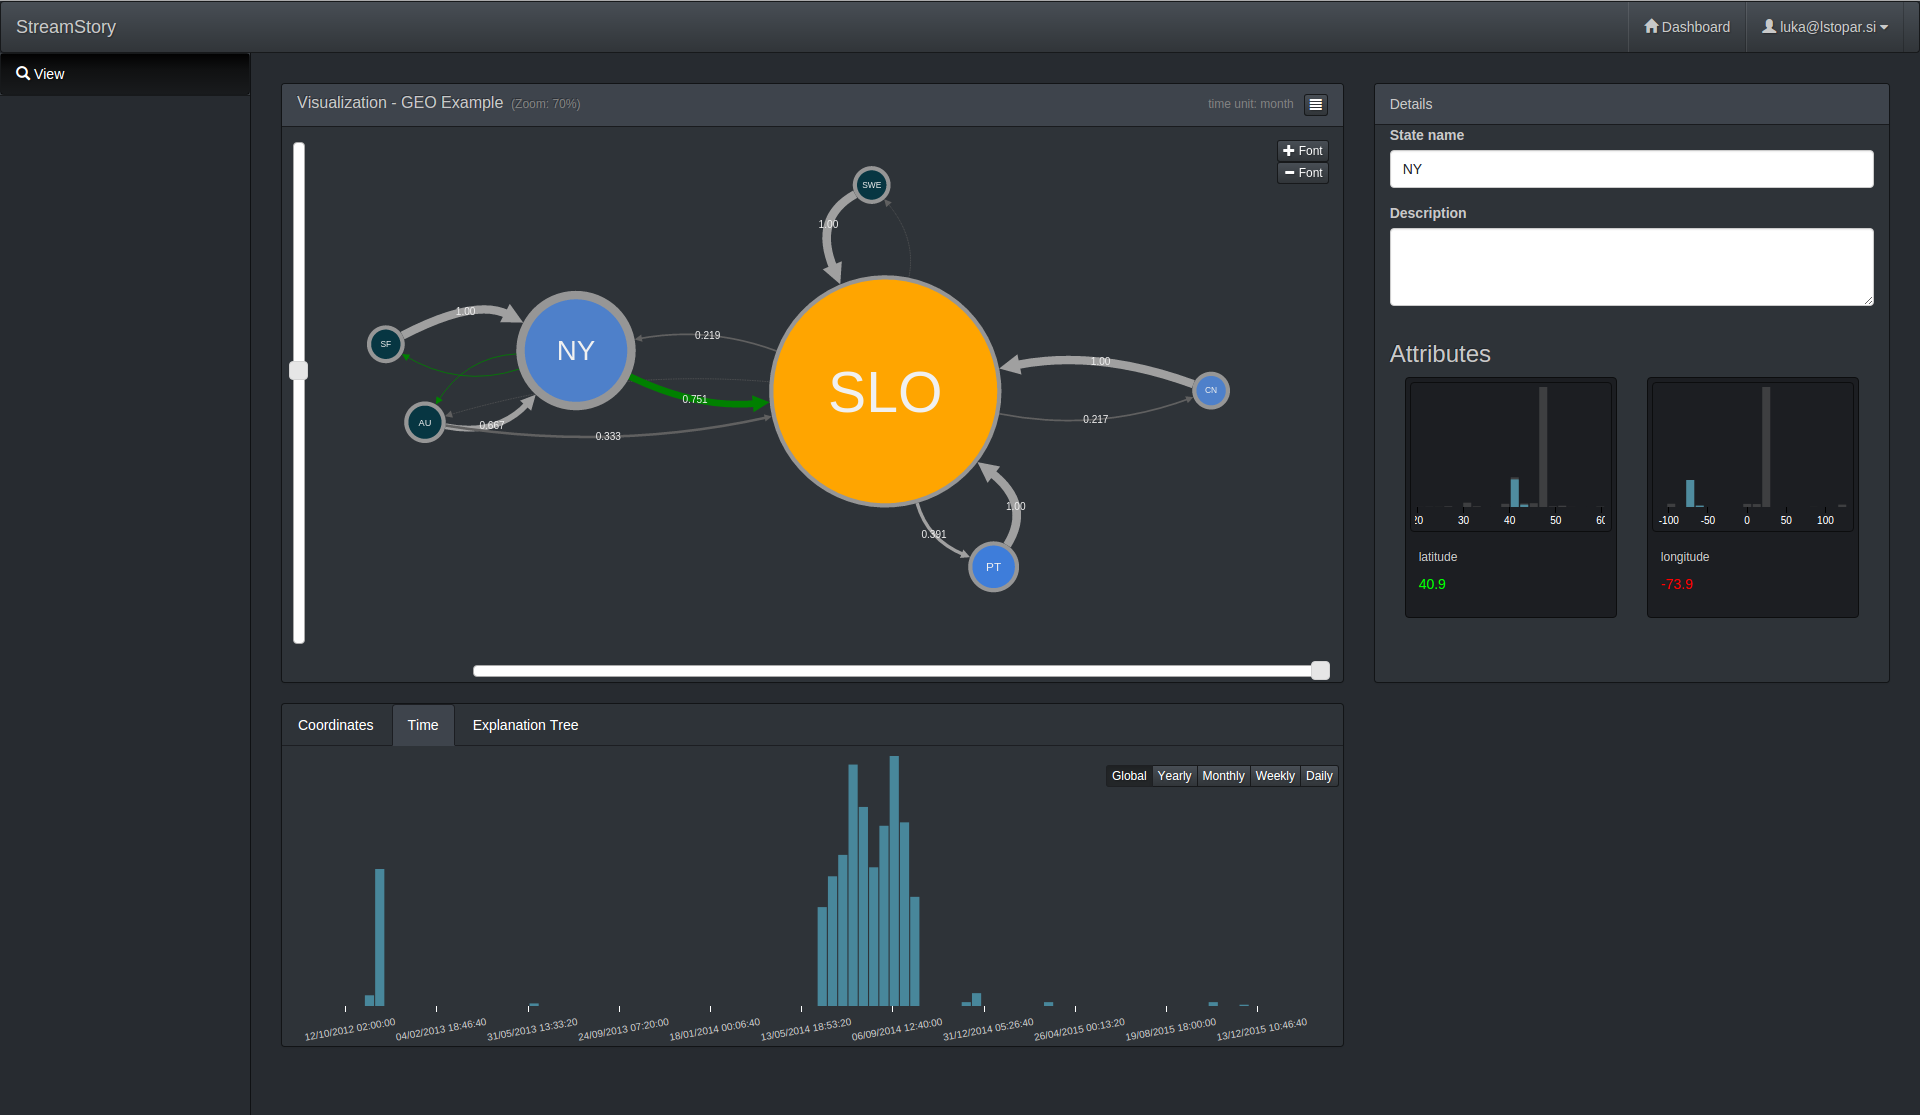
\includegraphics[width=16cm]{teaser}
	\caption{On the move: yearly travels of a European researcher.}
}

%% Uncomment below to disable the manuscript note
%\renewcommand{\manuscriptnotetxt}{}

%% Copyright space is enabled by default as required by guidelines.
%% It is disabled by the 'review' option or via the following command:
% \nocopyrightspace

%%%%%%%%%%%%%%%%%%%%%%%%%%%%%%%%%%%%%%%%%%%%%%%%%%%%%%%%%%%%%%%%
%%%%%%%%%%%%%%%%%%%%%% START OF THE PAPER %%%%%%%%%%%%%%%%%%%%%%
%%%%%%%%%%%%%%%%%%%%%%%%%%%%%%%%%%%%%%%%%%%%%%%%%%%%%%%%%%%%%%%%%

\begin{document}

%% The ``\maketitle'' command must be the first command after the
%% ``\begin{document}'' command. It prepares and prints the title block.
\firstsection{Introduction}

\maketitle

%% the only exception to this rule is the \firstsection command
%\section{Introduction}
\label{sec:introduction}
The visualization of multivariate time series is a challenging task. Often, systems are observed through one-dimensional measurements graphed over time. Modern systems often have many different sensors which 
typically operate in approximate cycles over time. Typical examples include weather systems (e.g. the seasons), manufacturing systems and power consumption. 
%
In this paper, we  present the StreamStory system for analyzing and visualizing multi-variate time series with minimal prior knowledge of the underlying time series. One of the key features of our system is that it allows for  \emph{multi-scale analysis} of the underlying system allowing the user to interactively find suitable scales to interpret \primoz{the multivariate}\lstopar{their} data in a qualitative representation.  

Intuitively, the system helps users detect behaviors which map to conceptual states of the system. For example, in the case of weather, a ``summer'' state may include higher average temperatures, while a ``winter" state would have lower temperatures. 
%
This representation is built using the following pipeline. First, we capture the structure of the data by employing unsupervised machine learning
techniques to identify the systems' most typical states. Next, we capture the
dynamics by modeling transitions between these states using a Markov chain framework.
Finally, we construct a hierarchical representation by aggregating both
states and transitions. Each level of the hierarchy is then associated with a unique
scale or detail level.

Overall, this system gives the user a hierarchical view of the dynamics as well as 
allow for analysis of the system. After the initial model is built, we visualize the model
in a web-based user interface, (see Figure 1), allowing the 
user to zoom between scales interactively. To help users identify the
meaning of states and transitions, the system provides several automatic assistance services,
including automatic state labeling, rule extraction, attribute highlighting which
identify \emph{differences in states}, as well as several tools to help visualize an individual states'
structure. 
%
The system provides additional helper  services based on the Markov chain model. It can map online streaming data onto 
the model in real-time and issue alerts and messages based on parameters set in the interface. %This can be useful in several scenarios we describe in the paper.
%
The main technical contributions of the paper are
\begin{enumerate}{}
  \item A novel methodology for modeling and visualizing multivariate time-varying data streams. This approach is able to capture multiscale behaviour by building a hierarchical model of the system. We use Markov chains to visualize the dynamics of a system and propose an algorithm for constructing hierarchies of recurrent continuous time Markov chains, which preserves stationary distributions and has not appeared in the literature. %We also design our method to preserve as much of the dynamics as possible throughout the hierarchy.
  \item Building on these ideas, we develop and implement an interactive system which incorporates many different features to help analyze and understand complex systems through our visualization tool (\url{http://streamstory.ijs.si}).
  \item The system provides functionality to process and visualize online streaming data and provide \primoz{a}\lstopar{the} user with  alerts and messages on identified behaviours in the system.  
\end{enumerate}

% The paper is structured as follows. Section \ref{sec:previous} provides and overview
% of visualization tools used for data exploration and the state-of-the-art in using Markov chains for modelling dynamic systems.
% Section \ref{sec:preliminaries} introduces the concepts and notations used throughout the paper and 
% in sections \ref{sec:multiscale-framework} and \ref{sec:multiscale-implementation}, we present
% our multi-scale methodology and the details of its implementation. We then present some of the 
% features of our user interface in Section \ref{sec:ui}. We then show experiments conducted on real-world datasets in Section \ref{sec:experiments} and conclude with a discussion and further work in Section \ref{sec:discussion}.

\begin{comment}
These 
systems include, for example, the solar system, manufacturing systems or weather 
systems. Such systems can be characterized by a set of states, along with associated
state transitions. States, on a high level, may include a ``sunny" state and a ``rainy"
state or maybe states with high and low productivity. For example, when a pilot wishes
to change an aircrafts heading, they will put the aircraft into state ``banking turn"
by lowering one aileron and raising the other, causing the aircraft to perform a
circular arc. After some time, the wings of the aircraft will be brought level by
an opposing motion of the ailerons and the aircraft will go back into state "level".

Such high-level states can be decomposed into lower-level states, giving us a 
multi-scale view of the system and allowing us to observe the system on multiple 
\lstopar{detail levels}. For example, a "banking turn" state can be decomposed by the
aircrafts roll and angular velocity, resulting in perhaps three states: "initiate
turn", "full turn" and "end turn".

In this paper we present a methodology for modeling and visualization of such systems and demonstrate its implementation
called StreamStory. StreamStory is a tool for summarizing multivariate continuously
time-varying data streams in a qualitative manner on multiple scales, by representing the system with 
its most typical states and their associated transitions and aggregating them to obtain
a hierarchical representation.

To achieve such a representation, we propose a three step methodology. In the first
step we capture the structure of the data by employing unsupervised machine learning
techniques to identify the systems' most typical states. The second step captures
dynamics by modeling transitions between these states using a Markov chain framework.
The third and final step constructs a hierarchical representation by aggregating
states and transitions. Each level of the hierarchy is then associated with a unique
scale or detail level.

We visualize this hierarchical model in a web-based user interface, shown in \lstopar{Figure} \ref{fig:teaser}.
The user interface is designed to show the model on a single scale and allows users
to switch scales using the zoom function. To assist users in identifying the
meaning of states and transitions we developed several automatic assistance services,
from automatic state labeling, rule extraction and attribute highlighting which
identify \lstopar{differences in states}, to various histograms that show the states'
structure.



\iffalse
\lstopar{a to obdrzimo? Furthermore, we divide the inputs streams into two sets: observation and control set.
Attributes in the observation set are the attributes that tell us the state of the 
system and, we assume, cannot directly influence its dynamics. These are parameters
that users cannot directly manipulate, like aircraft tilt from the previous example,
which must be indirectly manipulated through the angles of ailerons. We use observation
attributes to identify, and aggregate, low-level states, detect outliers (anomalies) 
and determine the current state of the system.}
\fi

\iffalse
In contrast, users can directly manipulate attributes in the control set. These 
are attributes like angles of ailerons that may directly influence the behavior 
(observation attributes) and performance of the system. For example, when an operator 
in a steel factory sets the cooling temperature to a high value, the product will
take longer to go from state "hot" to state "cool". As such, we assume, control attributes
may influence the occurrence, and expected time, of undesired states, associated with
undesired events.
\fi

\iffalse
Our system uses control attributes to model state transitions, allowing us to observe
the dynamics with respect to the current configuration and gives us insight into the
expected dynamics with respect to some alternate attribute configuration.
\fi

\lstopar{The main research contributions presented in this paper can be summarized as follows:
\begin{enumerate}{}
  \item We present a novel methodology for modeling multivariate continuously time-varying data streams
  in a hierarchical manner providing a unique model of the several detail levels.
  \item We present a novel approach for modeling state transitions in a Markov chain allowing
  to observe the dynamics of the chain under alternate configurations.
  \item We propose a recursive algorithm for partitioning recurrent continuous time Markov chains.
  \item \lstopar{Exploratory Data Analysis Tool}
\end{enumerate}
}

The remainder of this paper is structured as follows. Section \ref{sec:previous} provides and overview
of visualization tools used for data exploration and the state-of-the-art in Markov chain research.
Sections \ref{sec:preliminaries} introduces the concepts and notations used throughout the paper.
In sections \ref{sec:multiscale-framework} and \ref{sec:multiscale-implementation} we present
our multi-scale methodology and the details of its implementation. We then present some of the 
features of our user interface in Section \ref{sec:ui} and some implementation details in Section
\ref{sec:implementation}. We then show experiments conducted on real-world datasets in Section \ref{sec:experiments}
and \lstopar{provide a discussion with some general thoughts on further work} in Section \ref{sec:discussion}.

\end{comment}


%% \section{Introduction} %for journal use above \firstsection{..} instead


\section{Previous Work}
\label{sec:previous}
Large multivariate datasets have become common in many applications, including production lines,
monitoring systems, bioinformatics and social sciences. As the number of observations increases,
existing tools become cluttered and unresponsive. This clutter saturates visualization and hinders
data analysts as large response times make interactive exploration difficult.

Many techniques have been proposed in the literature that address this scalability problem.
They can generally be classified into two groups: data abstraction and clutter reduction 
techniques.

Techniques for data abstraction used in visualization include filtering [TODO cite], clustering
and sampling [TODO cite].

Clutter reduction assigns more space to interesting data and tries to hide less interesting data.
The most common techniques for clutter reduction include zooming and distortion.

This section starts by providing the state-of-the-art in clustering and Markov chain research and
then continues with an overview of existing visualization techniques.

\subsection{General Visualization Techniques}

Shneiderman \cite{545307} proposes a task-by-data-type taxonomy of information visualizations of multi-dimensional
data types as well as structured data which provides researchers and developers with a guideline for
the design and implementation of visualization systems. His work highlights the importance of data
abstraction operations such as summarization, filtering, zooming and extraction.

Jeong and Pang \cite{729555} present a technique called reconfigurable disc trees for visualizing large 
hierarchical data sets. The data is presented as a tree which can be laid out in two or three dimensions.
Their visualization is based on discs around which the children of each node are placed and eliminates
visual overlaps among subtrees.

Johnson and Shneiderman \cite{Johnson:1991:TSA:949607.949654} present another technique for visualizing hierarchical
information called TreeMaps. TreeMaps recursively partition the display into rectangular bounding boxes representing the 
tree structure. The drawing of nodes within their bounding box is dependent on their content and can be interactively
controlled.

Fua et. al. \cite{Fua:2000:SBM:614278.614457} present a mechanism for navigating hierarchically organized structures
called Structure-Based brushes. Brushing consists of painting sections of the display using a mouse or stylus, indicating
data items to be selected. Their technique can be used to perform selection in datasets organized via hierarchical
clustering and partitioning algorithms and serves to perform subset selection for further analysis. The technique defines
the level of detail which can be e.g. the cluster size, volume of the level number which can be used to traverse the
hierarchy.

\subsection{Visualization in Data Mining}

Visualization is an important tool in data mining as it \textcolor{red}{...}. Data mining is commonly defined
as the extraction of patterns or models from data sets, usually as part of extracting high-level
knowledge from low-level data. Visualization is an important tool in this area as it gives analysts a
tool for exploring, understanding data and creating hypothesis.

Visualization techniques used in data mining range from simple techniques for data exploration, such as
scatter plots, box plots, heatmaps, etc., to visualization of more complex structures such as PCA [TODO cite],
association rules, decision trees [TODO cite], clusters and dendrograms.

Oliveira and Levkowitz \cite{1207445} provide a survey of visualization tools used for data mining. Their survey focuses
to visualization of tabular data and provides an overview of tools and techniques for data exploration,
visualization of the extracted knowledge, discussing the question of how to select an appropriate visualization
technique.

Keim \cite{981847} provides a classification of information visualization techniques used in data mining, which is based on
the data type, visualization technique and interaction and distortion technique.

\subsection{Markov Chains}

Hierarchical structures are used in many real-world applications, as they are flexible in storing information
and allow the user to zoom into detail high detail levels, while hiding these details on the upper levels.

\begin{itemize}
	\item \cite{5746509} present a recursive bi-partitioning algorithm for partitioning discrete-time Markov chains. The 
	algorithm uses Kullback-Leibler divergence rate to measure the difference between the original Markov
	model and the its approximation. The authors also present a formula for aggregating states in the discrete-time
	Markov chain.
	
	\item \cite{pande-beauchamp-bowman:2010:methods:markov-model-review} present an overview of using Markov chain models in the bio-chemical domain. The paper
	presents approaches for modeling states (assigning observations to states) as well as building a transition
	matrix (using counts). The authors mention that to improve transition estimation one can use Bayesian priors.
	For example a prior that includes the effect of detailed balance can enhance the effectiveness when dealing with
	small counts. The authors also mention simplifying the transition matrix into fewer states by looking at larger
	timescales. This is done by spectral clustering.
	
	\item \cite{Benz2004239} present a multi-resolution framework for analysis of image data by exploring a hierarchical
	image object network and representing strongly linked objects, using polygons and fuzzy systems.
	
	\item \cite{4015421} Investigate data abstraction quality measures in multiresolution visualization systems. Spcifically, they propose
	a histogram difference measure and a Nearest neighbor measure to measure the quality of the abstraction.
	
	\item \textcolor{red}{[TODO Bertini and Santucci [7] present a quality measure for sampling and apply it to finding the optimal sampling level]}
	
	\item \textcolor{red}{Hierarchical Parallel Coordinates}

	\item \cite{Elmqvist:2010:HAI:1749404.1749525}
	present a model for building, visualizing and interacting with multi-scale representations of visual information
	using hierarchical aggregation. Their work presents a model for transforming visualization techniques into a multiscale
	structure using hierarchical aggregation.
	
	Like their model, we also aggregate information in the data space.
	
	\item \textcolor{red}{Venn diagrams}
	
	\item \textcolor{red}{Categorical (hierarchical view)} [v brushes reference [12], [14]]
\end{itemize}

\textcolor{red}{We differ from the related work in that we summarize the information, instead of drawing the whole
dataset. We also summarize the dynamics of the dataset.}

\section{Preliminaries}
\label{sec:preliminaries}
Our framework is aimed at visualizing multivariate time-series. Here we introduce the tools required in our framework. We assume as input we are given samples of $d$ signals, which we interpret as one multi-dimensional signal:
$$f: x(t)\mapsto \R^d$$
For simplicity, we assume that the signals are continuous and real-valued as well as uniformly sampled. This means that all signals are sampled simultaneously and at constant intervals. These assumptions can be relaxed in practice, with a preprocessing resampling step.  Each sample then consists of a vector of samples from all input signals at time $t$. If our system is intrinsically $d$-dimnesional, then by Whitney's embedding theorem, if we have $2d+1$ independent signals, we should be able to reconstruct the system.

If we do not have enough independent signals, we can always use a time-delay embedding to raise the dimension of our signal using Takens embedding theorem \cite{} and extensions \cite{}.  

A time-delay embedding is defined as a function:
$$ f(x(t),d,\tau) = (x(t),x(t+\tau),\ldots,x(t+(d-1)\tau) )$$
It takes a times series and lifts it to $d$ dimensions by considering samples spaced at $\tau$ intervals. There is considerable amount of work on how to choose $\tau$, but in our case we often (a) have sufficiently many signals (b) almost any value of $\tau$ works. 

From this point on we  assume that the image of $f$ defines a compact subset of Euclidean space. For our input, we assume a PL-reconstruction based on time-adjacent samples. \primoz{(maybe an example here?)}

Our main modelling tool is the continuous time Markov chain (CTMC). Markov processes are a special kind of stochastic processes with the characteristic of  	having no memory. This means that only the current state of the process can influence	where the process goes next \cite{norris1998markov}. In this work we focus on a special kind
	of Markov processes called Markov chains that can assume only a finite or countable
	number of states.

Markov chains can be used to model many phenomena of interest and have been used in many
	applications, including [TODO]. What makes them particularly useful is that the memoryless
	property makes it feasible to predict future developments and compute probabilities and
	expected values to quantify that behavior.
	
	More formally, a Markov chain is a stochastic process $(X_t)_{t \ge 0}$ which we assume has 
	only a finite or countable number of states $i \in I$. The starting state
	is sampled from a probability distribution $\lambda$, called the initial distribution.
	We define $p_{ij}(t)$ to be the probability of the process being in state $j$ at time $t$
	when starting from state $i$ at time $0$ and a stochastic matrix $P(t)$, where $\left(P(i)\right)_{ij} = p_{ij}(t)$.
	Each row of $P(t)$ is thus a probability distribution over the state space $I$. In our
	work we assume that $P(t)$ is recurrent for every $t$ and that the process is non-explosive.
	
	The literature distinguishes between two types of Markov chains: discrete time and continuous time.
	Discrete time Markov chains are the most basic type of Markov chains, where the process
	changes states in discrete time steps $n \in \mathbb{N}$ with probabilities $p_{ij} = p_{ij}(1)$
	and obeys the Markov property presented in Definition \ref{thm:markov-property-discrete}.
	
	\begin{defn}
	\label{thm:markov-property-discrete}
	Let $(X_n)_{n \ge 0}$ be a discrete time Markov chain with initial distribution $\lambda$.
	Then conditional on $X_m = i$, $(X_{m + n})_{n \ge 0}$ is also a Markov chain with initial
	distribution $\delta_i$ and is independent of $X_0, X_1, ..., X_m$.
	\end{defn}
	
	Continuous time Markov chains are a generalization of discrete time Markov chains as they
	gap between the discrete time steps is filled and the process can change states at any given moment.
	Continuous time Markov chains are closely related to Poisson processes. Imagine the state
	space $I$ as a labyrinth of corridors and chambers. The corridor between chambers $i$ and $j$
	is shut by a single door that opens for an infinitely small amount of time at the jump times of
	a Poisson process with rate $q_{ij}$. If the person walking through the labyrinth changes
	chambers each time a door opens, they are performing
	a continuous time Markov chain.

	\primoz{formal defintion and reference} 
	
	The basic data needed to define a continuous time Markov chain on state space $I$ are
	given by a transition rate matrix $Q$ satisfying the following conditions:
	
	\begin{enumerate}
		\item $q_{ij} \ge 0$ for all $i \ne j$
		\item $\sum_{j \in I} q_{ij} = 0$
		\item $-\infty < q_{ii} \le 0$ for all $i \in I$.
	\end{enumerate}
	
	Each off-diagonal element of $Q$, $q_{ij}$ represents the rate of jumping from state $i$ to state $j$,
	while the diagonal elements $q_{ii}$ represent the rate of leaving $i$. The stochastic matrix
	$P(t)$ is represented as $P(t) = e^{tQ}$ and can be computed by solving Kolmogorov's equations:
	\begin{equation}
		\frac{d}{dt}P(t) = P(t)Q
	\end{equation}
	with initial condition $P(0) = I$.


To go from our PL-input signal to a Markov chain, we consider a spatial discretization of the signal.
Let $S\subseteq \R^d$, be the support of our input signal. Given a partition of $S$, denoted by  $\cP$, 
we can construct a Markov chain. Construct a  state in a Markov chain $\cM_i \in \cM$ for each  partition cell $\cP_i$. Let this mapping be denoted by $f:\cP \rightarrow \cM$. We can endow our data with a canonical measure induced from the volume measure on $\R^{d+1}$ \primoz{here we have to be a bit careful about time}. This induces a measure on the partitions $\mu$, which by the  pushforward $f(\mu)$, induces a measure on the states. This represents the empirical stationary distribution on our Markov chain. To define the transition probabilities, we note that it can be defined in terms of the adjacent partition elements. \primoz{there are a few details to put in here} 

This completely defines a continuous time Markov chain. Here, we would like to note that this step represents the fundamental information loss in our approach. The transition from continuous process to discrete space (without memory) inherently loses information in any dimension larger than 1 (see Appendix).  

The Markov chain we obtain is highly dependent on the choice of partition. In principle, the initial discretization step  results in a relatively large Markov chain corresponding to a fine partition of the space. Our main contribution is to consider the Markov chains over multiple scales. This corresponds to a \emph{hierarchical partition of space}. From above, we have that any partition induces a Markov chain. 

If we are given a sequence of increasingly coarse paritions there is a well defined surjective map 
$\cP(i)\rightarrow\cP(j)$ from finer to coarser. Each such map also induces a well-defined map between Markov chains. \primoz{Can we prove that these are the same as what we do?}

In practice, we are not given a hierarchical partition of space, but rather using our initial Markov chain, we define a map between Markov chains by merging states. Note that any such sequence does correspond to a hierarchical partition. \primoz{Maybe add a two line proof here}.  In the following section, we describe how we compute the smaller Markov chain given an initial Markov chain and a map. We also describe how we choose which states to merge, but the intuition is to merge states so that as little of the underlying dynamics is lost. 

In section~\ref{}, we decribe how we constructed the underlying partition and our initial Markov chain.  


% hierarchical partitions of space

% maps between markov chains



\section{Multiscale Hierarchies - Framework}
\label{sec:multiscale-framework}
\iffalse
\begin{itemize}
	\item Initial state construction (State Identification)
	\item Aggregation (State Aggregation)
	\item Transition probabililties (Modeling transitions)
\end{itemize}
\fi

To capture and summarize the dynamics of the system our methodology represents the data
in a qualitative manner using states and transitions. We begin this section with an overview
of our multi-scale methodology. The methodology consists of three main steps and is
shown in Figure \ref{fig:methodology}.

\begin{figure}[h!]
	\centering
	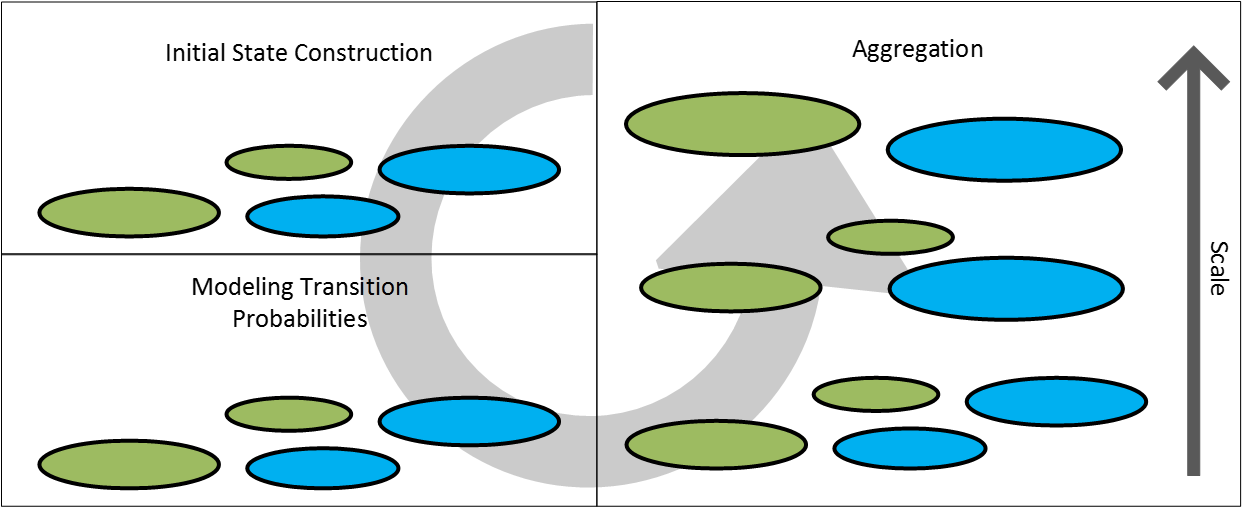
\includegraphics[width=\columnwidth]{methodology}
	\caption{\lstopar{TODO}}
	\label{fig:methodology}
\end{figure}
The methodology starts in the top left part of the figure with an initial step that summarizes
the structure of the data by identifying their most typical states. It achieves this by \lstopar{placing}
the data in a \lstopar{design time} metric space and partitioning them. It then associates
each partition with a single state.
\lstopar{
\begin{itemize}
	\item These states are used as the lowest-level states.
\end{itemize}
}
The methodology then moves in the counter clockwise direction. The second step summarizes
dynamics. It does so using the continuous time Markov chain framework presented in Section \ref{sec:preliminaries}.
The third and final step aggregates states and transitions into a hierarchy, associating each
level of the hierarchy with a unique scale, thus providing a multi-scale model. These steps 
are explained in detail in the next subsections.


\subsection{Initial State Construction}
\label{sec:framework-states}

The first step in our methodology is the construction of initial lowest level states. Using the notation
from Section \ref{sec:preliminaries} we define a partition function 
from $\lstopar{f}: \mathbb{R}^d \rightarrow I$ mapping the $d$-dimensional signal to lowest level states
\lstopar{
with the following properties:
\begin{itemize}
	\item similar points in $\mathbb{R}^d$ should be mapped to the same or neighboring partitions.
\end{itemize} 
}

\subsection{Modeling Transition Probabilities}
\label{sec:framework-transitions}

While we represent the states as described in Section \ref{sec:framework-states},
to model transitions we use the continuous-time Markov chain (CTMC) framework.
As mentioned in Section \ref{sec:preliminaries} all the data needed to represent a continuous-time Markov chain
is stored as transition rates in a transition rate matrix $Q \in \mathbb{R}^{n \times n}$, where $n$ represents
the size of the finite state space $I$. However, initial user
feedback showed transition rates are not a very informative way of visualizing state transitions. Therefore
we choose to visualize transitions in terms of the jump chain $\Pi$.
We note that an alternative way of representing a Markov chain $(X_t)_{t \ge 0}$ with transition rate matrix $Q$
is by its jump chain and holding times. The jump chain of a continuous time Markov chain $(X_t)_{t \ge 0}$ is
a discrete time Markov chain $(Y_n)_{n \ge 0}$ with transition matrix $\Pi$ defined as
\begin{equation}
	\nonumber
	\left(\Pi\right)_{ij} = 
		\left\{
			\begin{array}{ll}
				-\frac{q_{ij}}{q_{ii}} & \mbox{if } i \ne j, q_{ii} \ne 0 \\
				0 & \mbox{if } i \ne j, q_{ii} = 0
			\end{array}
		\right.
\end{equation}
\begin{equation}
	\nonumber
	\left(\Pi\right)_{ii} = 
		\left\{
			\begin{array}{ll}
				0 & \mbox{if } q_{ii} \ne 0 \\
				1 & \mbox{if } q_{ii} = 0
			\end{array}
		\right.
\end{equation}
Definition \ref{def:jump-chain-holding-times} provides a definition of a Markov chain in terms of its jump chain and holding times.

\begin{defn}
	\label{def:jump-chain-holding-times}
	A right-continuous process $(X_t)_{t \ge 0}$ is a continuous time Markov chain with initial
	distribution $\lambda$ and transition rate matrix $Q$ if its jump chain $(Y_n)_{n \ge 0}$ is a 
	discrete time Markov chain with initial distribution $\lambda$ and transition matrix $\Pi$ and
	for each $n \ge 1$, conditional on $Y_0, Y_1, ..., Y_{n-1}$, its holding times $S_1, S_2, ..., S_{n-1}$
	are independent exponentially distributed random variables of parameters $q_{Y_0}, q_{Y_1}, ..., q_{Y_{n-1}}$
	where $q_i = -q_{ii}$.
\end{defn}

To determine the size of each state, we turn to the ergodic properties of $(X_t)_{t \ge 0}$, specifically
we use the elements of the stationary distribution $\pi = (\pi_1, \pi_2, ..., \pi_n)$ and draw the area of
state $i$ proportional to $\pi_i$. We note that under the assumption presented in \ref{sec:preliminaries}
this distribution always exists.

\subsection{Aggregation}
\label{sec:framework-aggregation}

By the final step of our methodology, we have already computed a qualitative representation of the
dataset. The goal of the third step is then to construct a multi-scale representation, representing
the data in several details level - from the finest to the most coerce.

As stated in Section \ref{sec:preliminaries} we associate each scale $s$ with a specific partition
function $\lstopar{f_s}: \mathbb{R}^d \rightarrow \lstopar{I_s}$. At the finest scale, we use the 
partition function \lstopar{$f: A \rightarrow B$ [TODO the function]} as defined in Section \ref{sec:framework-states}, inducing state space $I$. We then compute the partition
function for coarser scales by aggregating elements in $\Ima \lstopar{f}$, inducing state space $I_s$.
Thus $I_s$ represents a partition of $I$ and is determined by a map $\phi_s: I \rightarrow I_s$. This
way $f_s$ can be represented as a compositum $f_s = f \circ \phi_s$.

We represent the Markov chain $(X_t^{(s)})_{t \ge 0}$ induced by state space $I_s$ with a transition
rate matrix $Q^{(s)}$. To compute $Q^{(s)}$, we adapt the formula
proposed in \cite{5746509} to continuous time Markov chains. We define a partition function
$\Phi: \mathbb{R}^{n \times n} \rightarrow \mathbb{R}^{m \times m}$ with $m \le n$ using formula \ref{eq:ctmc-state-aggregation}.
\begin{equation}
	\label{eq:ctmc-state-aggregation}
	\Phi(Q) = (P' \Pi P)^{-1} P' \Pi Q P
\end{equation}
where $\Pi = diag(\pi)$, $\pi$ is the stationary distribution of $(X_t)_{t \ge 0}$ and $P$ is a 
$n \times m$ matrix with elements
\begin{equation}
	\nonumber
	\left(P\right)_{ij} = 
		\left\{
			\begin{array}{ll}
				1 & \mbox{if } \phi(i) = j \\
				0 & \mbox{otherwise}.
			\end{array}
		\right.
\end{equation}
Thus the data needed to represent a Markov chain at a specific scale $s$ is obtained by applying \ref{eq:ctmc-state-aggregation}
is obtained as $Q^{(s)} = \Phi(Q)$.
If we define $\psi = \phi \circ \phi^{-1}$, then Equation \ref{eq:ctmc-state-aggregation} can be rewritten as
\begin{equation}
	\nonumber
	q_{\phi(i)\phi(j)}^{(s)} = \frac{\sum\limits_{i \in \psi(i)}\pi_i \sum\limits_{j \in \psi(j)} q_{ij}}{\sum\limits_{i \in \psi(i)}\pi_i}
\end{equation}
We note that $\pi^{(s)}$, the stationary distribution of $(X_t^{(s)})_{t \ge 0}$, can be computed directly from
the stationary distribution of the original chain $(X_t)_{t \ge 0}$ by the following rule:
\begin{equation}
	\nonumber
	\pi^{(s)} = \pi P
\end{equation}

\iffalse
\newpage

Once we have computed the lowest level Markov chain $(X_t)_{t \ge 0}$, we need to be able to represent it on multiple scales.
As stated in Section \ref{sec:preliminaries} we associate each scale $s$ with a specific partition function
$\lstopar{f_s}: \mathbb{R}^d \rightarrow \lstopar{I_s}$ where coarser partitions are generated by merging 
states of finer partitions.
Suppose we have already computed the finest level partition $\lstopar{\cP}$, inducing state space $I$ and the
coarser partition at scale $\lstopar{\cP_s}$, inducing state space $J$. Suppose the finest level Markov chain,
on state space $I$ is represented by a transition rate matrix $Q$ and define a surjective partition function
$\phi: I \rightarrow J$. To compute the Markov chain induced by state space $J$, we adapt a formula proposed
in \cite{5746509} to continuous time Markov chains. We define a partition function
$\Phi: \mathbb{R}^{n \times n} \rightarrow \mathbb{R}^{m \times m}$ with $m \le n$ using formula \ref{eq:ctmc-state-aggregation}.
\begin{equation}
	\label{eq:ctmc-state-aggregation}
	\Phi(Q) = \tilde{Q} = (P' \Pi P)^{-1} P' \Pi Q P
\end{equation}
where $\Pi = diag(\pi)$, $\pi$ is the stationary distribution of $(X_t)_{t \ge 0}$ and $P$ is a 
$n \times m$ matrix with elements
\begin{equation}
	\nonumber
	\left(P\right)_{ij} = 
		\left\{
			\begin{array}{ll}
				1 & \mbox{if } \phi(i) = j \\
				0 & \mbox{otherwise}.
			\end{array}
		\right.
\end{equation}
If we define $\psi = \phi \circ \phi^{-1}$, then Equation \ref{eq:ctmc-state-aggregation} can be rewritten as
\begin{equation}
	\nonumber
	\tilde{q}_{\phi(i)\phi(j)} = \frac{\sum\limits_{i \in \psi(i)}\pi_i \sum\limits_{j \in \psi(j)} q_{ij}}{\sum\limits_{i \in \psi(i)}\pi_i}
\end{equation}
\fi


\section{Multiscale Hierarchies - Implementation}
\label{sec:multiscale-implementation}
This section presents the implementation of our three step methodology presented in Section \ref{sec:multiscale-framework}.
We start by describing the methods behind the initial state construction in Section \ref{sec:state-construction-impl}
and then continue to present implementation details of steps two and three in sections \ref{sec:transition-probs-impl}
and \ref{sec:state-aggregation-impl} respectively.

\subsection{Initial State Construction}
\label{sec:state-construction-impl}

As described in section \ref{sec:framework-states} the initial state construction is performed by partitioning
the data points and associating each partition with a single state. The literature suggests many partitioning
algorithms, including those that produce a hierarchical partition. The computational complexity of these algorithms
is, however $O(n^2)$, rendering them unsuitable for large datasets.

To avoid this computational cost, we first create a flat partition of the data space and later aggregate these
partitions to obtain a hierarchical structure.

Following the intuition of Section \ref{sec:framework-states} we consider two data points similar if they lie close
to each other in Euclidean space. \lstopar{Other distance measures are also possible but are out of scope of this paper.}
We use either K-Means or DP-means \cite{DBLP:journals/corr/abs-1111-0352} to construct the partition, representing each 
partition as a Voronoi cell around its centroid. When using StreamStory in real time, the current state is thus
selected by assigning the current sample to the nearest centroid using the following formula:
\begin{equation}
	\nonumber
	i = \argmin_{i \in \mathbb{N}_k} \|x - \mu_i\|.
\end{equation}

We note that the number of centroids (in case of K-Means) or the cluster radius (in case of DP-means) should
be chosen based on domain knowledge and the level of detail the user desires. This parameter also effects the 
initial model construction time as demonstrated in Section \ref{sec:implementation}.

\subsection{Modeling Transition Probabilities}
\label{sec:transition-probs-impl}

As described in Section \ref{sec:framework-transitions} we model state transitions using the continuous
time Markov chain framework, first presented in Section \ref{sec:preliminaries}. The transitions are 
modeled on the finest scale and are then aggregated using the formula presented in Section \ref{sec:framework-aggregation}.

We allow users to select a subset of attributes which are used to model transition rates. Since the
jump process from state $i$ to state $j$ can be characterized as a Poisson process, we can model its
transition rate $q_{ij}$ as a function of these attributes $q_{ij} = q_{ij}(x)$. We do this by first
discretizing the continuous time parameter into a discrete sequence $(0, \epsilon, 2\epsilon, ...)$,
estimating the transition rates as
\begin{equation}
	q_{ij}(x) = \frac{\epsilon}{\tilde{p}_{ij}(x)}
\end{equation}
where $\tilde{p}_{ij}$ is the estimated probability of jumping from state $i$ to state $j$ in time
$\epsilon$.

Suppose the process is in state $i$ at time $t$ and define a random variable $J_i = j \Leftrightarrow X_{t + \epsilon} = j$.
$J_i$ then has a multinomial distribution with parameters $(p_{i1}, p_{i1}, ..., p_{in})$ which can be 
modeled using a nominal logistic regression model \cite{glm-introduction} to estimate $\tilde{p}_{ij}(x)$.
The transition rate matrix is then constructed on-the-fly from a matrix of logistic regression models.

\lstopar{
We need to explain why modeling transitions using signals is useful and why it is used.
In previous documents I went on blabbering that by modeling transitions this way, we allow
the possibility of users observing the dynamics in alternate configurations and simulating
what would happen if they changed some parameter. (This was more or less BS though)
}

\subsection{Aggregation}
\label{sec:state-aggregation-impl}

With a fine partition already available, our methodology merges partitions to obtain a hierarchical structure.
We employ agglomerative clustering \cite{Murtagh83} producing a hierarchical partition structure.
Agglomerative clustering works by initially treating each partition as a singleton and then recursively
merging pairs of partitions until only a single partition remains.

The partitions chosen for merging are chosen based on some distance or similarity metric. In each step
the closes two partitions with respect to the chosen metric are merged. The results of an agglomerative clustering
algorithm is typically visualized as a dendrogram. Each merge is associated with a horizontal line, while
the $y$ coordinate of the line is the distance between the merged items. Similarly
we use this distance do define the scale on which a particular partition (state) lives. Figure \ref{fig:dendrogram} shows
the relationship between a dendrogram and \lstopar{our visualization}.

\begin{figure}[h!]
	\centering
	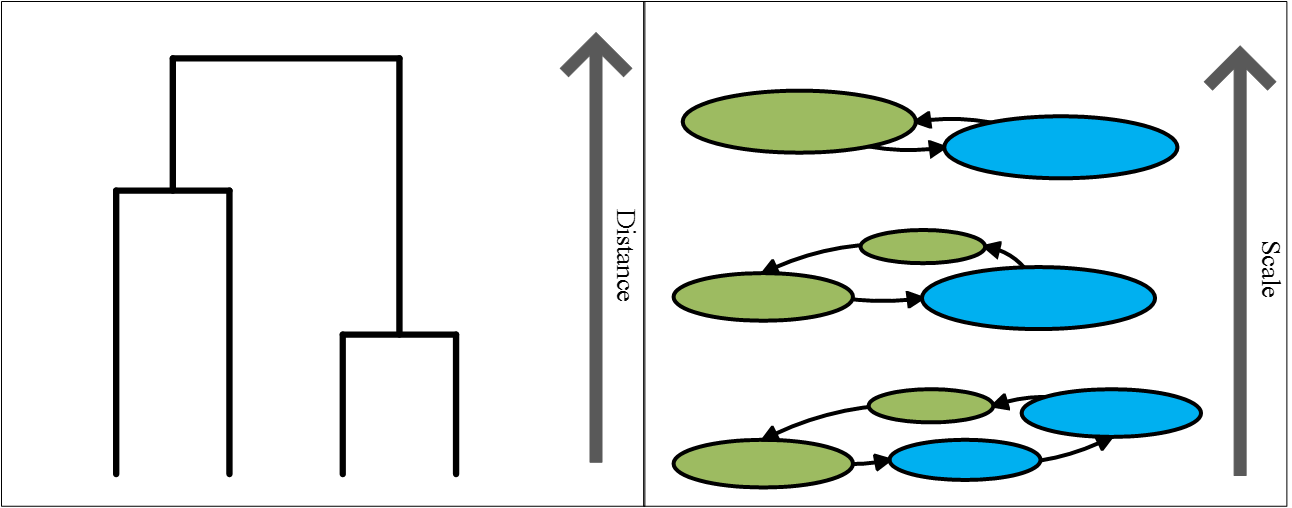
\includegraphics[width=\columnwidth]{dendrogram}
	\caption{\lstopar{TODO}}
	\label{fig:dendrogram}
\end{figure}

Along with a distance metric, agglomerative clustering also uses a design time linkage criteria, which determines
the distance between \lstopar{clusters} as a function of the pairwise distances between their elements. The most popular
linkage strategies in the literature are: single-linkage, complete-linkage and average (or mean) linkage. Our
experiments show no significant difference between the strategies.


\section{User Interface}
\label{sec:ui}

% \iffalse
% Features  
% \begin{itemize}
% 	\item Qualitative representation - states and transitions
% 	\item State identification services:
% 	\begin{itemize}
% 		\item State details and attribute highlighting - histograms + attribute colors
% 		\item \lstopar{Timeline + parallel coordinates \cite{parcoords} - when do states occur in time}
% 		\item \lstopar{Coloring states based on attributes}
% 		\item Decision trees + rule extraction - Explanation of states
% 		\item Automatic name generation
% 		\item Zooming into a state + showing paths from a state
% 	\end{itemize}
% \end{itemize}
% \fi

% \dunja{This needs a one sentence intro on the overall user interface.}
The user interface supports multiple views and features to help with exploratory analysis of data. For an overview of available functionality, see the supplementary video. A live system with the examples in this paper is publicly available for testing at \url{http://streamstory.ijs.si} - see supplementary material for details. 
The system supports multiple users with datasets and precomputed models (as well as the ability to store new models in the system). Data may be uploaded via CSV files.  Configuration consists of choice of desired attributes,  clustering method, aggregation strategy and attributes used to model transitions. The model is then constructed and the user can begin interactive exploration. The construction time varies depending on the size of 
their dataset and configuration. %We conducted an experiment to test the performance of our \lstopar{methodology},
%presented in section \ref{sec:implementation}.

The interface displays the model using a three panel user interface, an example of
which is shown in Figure \ref{fig:teaser}. Note that for the paper, we used a white background, whereas the default theme in the live system is with a dark background. The central panel visualizes the model at the current scale as a graph. A state is represented by a circle  whose size represents the time/probability spent in the state, which is computed from the stationary distribution of the Markov chain. The transitions are represented by arrows, where again size represents the empirical transition probability. 

% \iffalse
% Features  
% \begin{itemize}
% 	\item Qualitative representation - states and transitions
% 	\item State identification services:
% 	\begin{itemize}
% 		\item State details and attribute highlighting - histograms + attribute colors
% 		\item \lstopar{Timeline + parallel coordinates \cite{parcoords} - when do states occur in time}
% 		\item \lstopar{Coloring states based on attributes}
% 		\item Decision trees + rule extraction - Explanation of states
% 		\item Automatic name generation
% 		\item Zooming into a state + showing paths from a state
% 	\end{itemize}
% \end{itemize}
% \fi

% \dunja{This needs a one sentence intro on the overall user interface.}
% \lstopar{This section presents some of the key features of our three-panel web-based user interface.}
% The system supports multiple users with datasets and precomputed models (as well as the ability to store new models in the system). Data is generally uploaded via CSV files.  Configuration consists of choice of desired attributes,  clustering method, aggregation strategy and attributes used to model transitions. The model is then constructed and the user can begin interactive exploration. The construction time varies depending on the size of 
% their dataset and configuration. We conducted an experiment to test the performance of our \lstopar{methodology},
% presented in section \ref{sec:implementation}.

% The interface displays the model using a three panel user interface, an example of
% which is shown in Figure \ref{fig:teaser}. The central panel visualizes the model at the current scale as a graph. A state is represented by a circle  whose size represents the time/probability spent in the state, which is computed from the stationary distribution of the Markov chain. The transitions are represented by arrows, where again size represents the empirical transition probability. 
% >>>>>>> 63d0bf3dc78f345a11678b38161d979d0e825dc3

The computed model may be used as a monitoring tool, mapping incoming data onto the model in real-time. 
In this mode, the current state (green) and the most likely future states (blue)
are highlighted. The current state is determined by assigning a sample to its nearest 
centroid, as presented in Section \ref{sec:multiscale-implementation}, and is updated in real-time as
data arrives into the system.

The model is initially presented on a coarse scale with only a handful
of states. Users can then explore the model by either traversing the scales using the zoom 
function, as well as isolate and explore individual states using the ``Zoom Into'' function. %, \lstopar{or explore the graph as a tree using the ``Show Path'' function}.

Visualizing a Markov chain as a graph may not be, in itself,  sufficiently informative. The system offers several 
visualizations which assist users in identifying the meaning of states. These range from automatic
state labeling, state histograms, attribute highlighting and timeline histograms to decision trees
which visualize the states' properties in a hierarchical manner and \lstopar{human readable rules, summarizing the trees}.
These services are shown when the user clicks on and selects a state. We describe these visualizations below.  

%and each transition with an arrow on the 
%central panel. The size of a state is calculated from the associated entry in the stationary distribution
%and is proportional to the fraction of time the system spends in the state. The thickness of each arrow
%is proportional to the associated transition probability. 

% The computed 
% When using the model as a
% monitoring tool, 
%After registering, the user is presented with a dashboard, where they can organize their models.
%If they wish to create a new model, they have to upload a CSV file with the dataset they would
%like to visualize. 
%They are then taken through a configuration form, where they select attributes,
%clustering method, aggregation strategy and attributes used to model transitions. When completing
%the form, their new model is constructed. 

%Once constructed, a StreamStory 

\subsection{Probability Distributions and Attribute Highlighting}

The most basic exploratory tool to help a user is to plot the distribution of data inside each state in the form of a histogram. When clicking on a state, the histograms of all the attributes are shown in the right-side panel like in Figure \ref{fig:teaser}. Context for each distribution is shown as a global distribution of that attribute in the background.

%
%To assist the users to distinguish between states, we highlight each attribute either green of red.
%The color is chosen based on how typical the attribute is for the state. 
To help users understand the  values of attributes within a state, the attributes are colored according to their typical values.  For example, a bright green
value indicates that the attribute typically  has a higher value in this state compared to other states, while
a bright red color suggests, this value is low compared to other states. An example of attribute 
highlighting can be seen in Figure \ref{fig:example-naming}.

The color is calculated in the initialization step by first classifying all the samples assigned to the state 
against samples assigned to other states using a logistic regression model. All possible features are  used in the 
classification. % are all the dimensions of the input signal, which correspond to all possible attributes. 
The final color is determined by extracting weights from the models and associating positive weights
with green and negative with red.

The users can also view the distribution of attributes across states, by selecting a specific attribute.
When doing so, the states are recolored based on the value of the selected attribute - again, green indicates
a high value, while red indicates a low value.

%%here

\subsection{Automatic State Labeling}

Abstract states are often uninformative. While the transitions between states gives us insight into the dynamics of the system, it fails to provide a comprehensive summary 
of the dataset. Our initial user evaluations showed that first time, non-technical users had difficulty interpreting unlabeled states. % and had difficulty executing even the simplest tasks like finding
%states with high temperature in example \ref{sec:experiments-weather}}.

To help alleviate this, the system provides an automatic, data-driven, labeling service. The service labels states using ${<attribute,value>}$ pairs based on the inner-state distribution of attributes. The attribute is selected as one of the input signals, while the displayed value is a descriptive level with values: lowest, low, mean, high and highest.

Both the attribute and the level used in the label are computed by comparing the inner-state attribute
distributions to the global attribute distributions. The attribute selected by the naming process is
the one with the lowest $p$-value of the inner-cluster $40$-th and $60$-th percentile. The level is
then determined according to the $p$-value. If the $p$-value is below $0.12$ the attribute is labeled
as lowest or highest, while if the $p$-value is below $0.25$ it is labeled low or high. If none of the
attributes achieve a $p$-value of $0.25$ the state is labeled as a mean state. An example of an automatic
label, along with the associated inner-state and global histogram is shown in Figure \ref{fig:example-naming}.

\begin{figure}[h!]
	\centering
	\begin{subfigure}{.48\columnwidth}
	  	\centering
	  	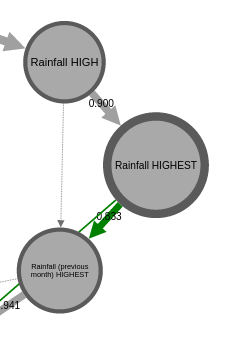
\includegraphics[width=0.7\columnwidth]{example-state-naming}
  		%\caption{\label{fig:example-naming-label}\lstopar{TODO}}
	\end{subfigure}
	\begin{subfigure}{.48\columnwidth}
	  	\centering
	  	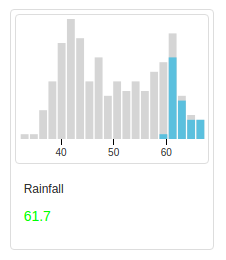
\includegraphics[width=\columnwidth]{example-state-naming-histogram}
	  	%\caption{\label{fig:example-naming-histogram}\lstopar{TODO}}
	\end{subfigure}
	\caption{Example output of the automatic state labeling service shown on the weather dataset presented in Section \ref{sec:experiments-weather}. The system labeled the bold state on the left hand side as "Rainfall HIGHEST", matching the inner-state distribution of rainfall shown on the right hand side.}
	\label{fig:example-naming}
\end{figure}

\iffalse
In order to assist the user in identifying the meaning of states, the system provides automatic default
state names, based on the distribution of attributes in the state. Each state is given a default name
by combining its most outstanding attribute with a discrete level: LOWEST, LOW, HIGH or
HIGHEST.

The attribute and the level are chosen by comparing its distribution inside the state to the global
distribution in all the states through histograms. This is achieved by first computing the percentiles
of the global distribution. The $40^{th}$ percentile is then computed for the state distribution and
compared against the global distribution. If this percentile lies below the $25^{th}$ or $12^{th}$
percentile, the state is marked with LOW or LOWEST respectively. The final name is chosen according
to the attribute which lies in the lowest percentile.
\fi

\subsection{Decision Trees and Rule Extraction}

An alternate description of states is generated through decision trees~\cite{Witten:2005:DMP:1205860}. Decision
trees are classification models often used in domains such as medicine for their explanatory power.
When a decision tree is induced, a splitting attribute and cut value are chosen recursively by a
design time criteria. The user can then interpret the tree by traversing the path from the root 
to one of the leafs.

Decision trees are provided as another tool for explaining states. We compute one tree for each
state by classifying the observations of the state against the observations of all other states,
obtaining a quantitative description of the state. We then extract rules from the decision tree,
providing a short summary of the state in the form of $A_i > t_i \cup A_j \in (t_{j_1}, t_{j_2}]$.

Figure \ref{fig:example-decision-tree-and-rule} shows an example decision tree and extracted rule
from a state in the weather dataset presented in section \ref{sec:experiments-weather}.

\begin{figure}[h!]
	\centering
	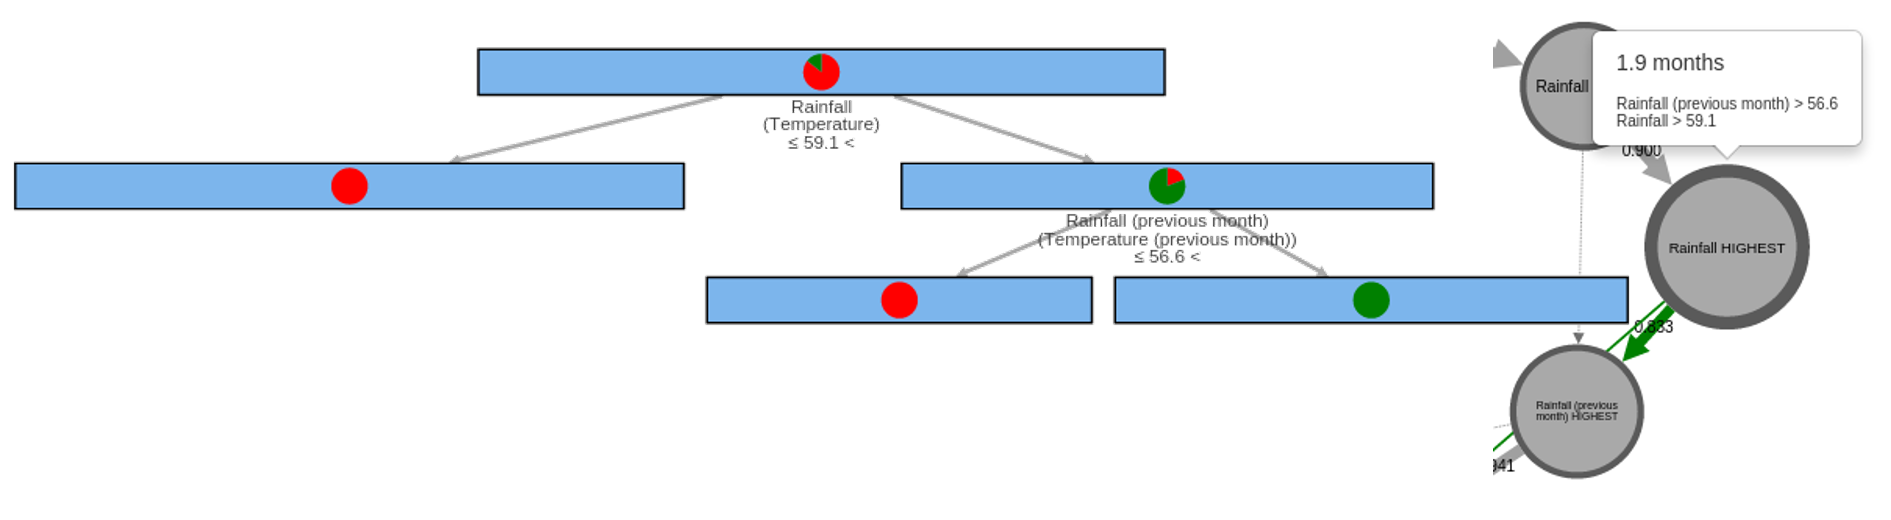
\includegraphics[width=\columnwidth]{example-tree-rule}
	\caption{Example output of a decision tree (left) and a rule (right) describing the summer state in the weather dataset presented in Section \ref{sec:experiments-weather}. We can see that the system describes the state as having rainfall over $59.1 mm$ and the previous month rainfall over $56.6 mm$ \lstopar{due to the high correlation between temperature and rainfall in the dataset}.}
	\label{fig:example-decision-tree-and-rule}
\end{figure}

\subsection{Streaming Data}

The system is also able to visualize streaming data based on a precomputed model. 
\lstopar{
By assigning each new data point to its nearest centroid on the finest scale and traversing the scales it allows
}
%Given a training set, the multiscale model is built. The system can then process the streaming data.
%For each new point, it determines its current state using on a nearest neighbor search to the centroids of the states. This is done at all scales, allowing
the user to visualize the current state and possible next states at different levels interactively. The system allows for alarms to be set to detect when the system enters a particular state or when the probability of entering a paraticular state exceeds some threshold. The probabilities are computed based on the Markov model at the scale at which the alarm is set 
(see Supplementary Video).

\iffalse
\begin{figure}[h!]
	\centering
	\begin{subfigure}{.3\columnwidth}
	  	\centering
	  	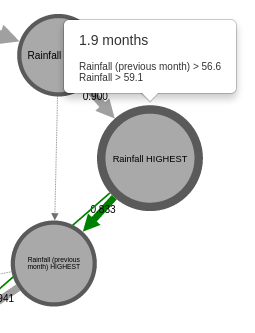
\includegraphics[width=\columnwidth]{example-rule}
%  		\caption{\lstopar{TODO}}
  		\label{fig:example-rule}
	\end{subfigure}
%	\begin{subfigure}{.68\columnwidth}
	\begin{subfigure}{0.9\columnwidth}
	  	\centering
	  	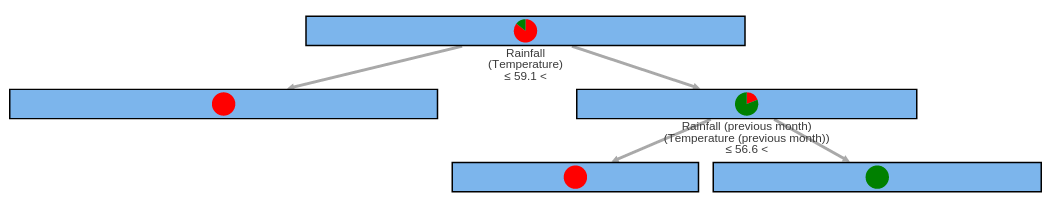
\includegraphics[width=\columnwidth]{example-decision-tree}
%	  	\caption{\lstopar{TODO}}
	  	\label{fig:example-decision-tree}
	\end{subfigure}
	\caption{Example output of a decision tree (right) and a rule (left) describing a state in the weather dataset presented in Section \ref{sec:experiments-weather}. We can see that the system describes the state as having rainfall over $59.1 mm$ and the previous month rainfall over $56.6 mm$.}
	\label{fig:example-decision-tree-and-rule}
\end{figure}
\fi

\iffalse

\subsection{Visual Assistance}

When a state becomes selected, the user interface presents the user with several visual aids which
assist them in identifying the states' meaning. The first of these aids is the timeline histogram
which shows the distribution of the states occurrence over time. An example is shown in Figure 
\ref{fig:time-hist}.

\begin{figure}[h!]
	\centering
	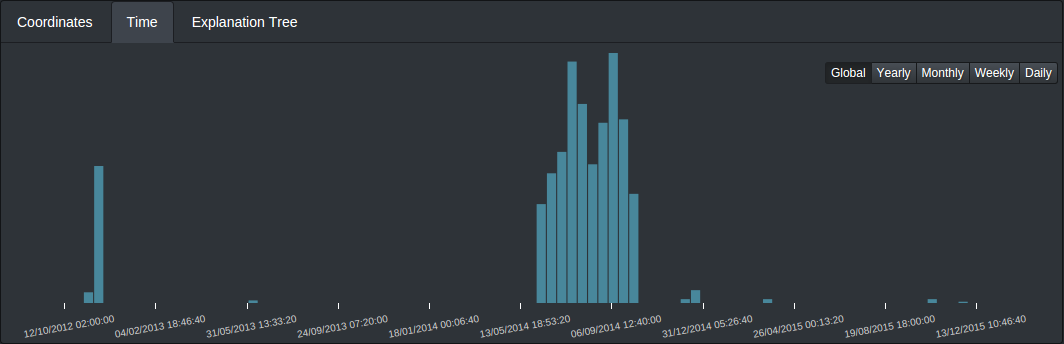
\includegraphics[width=\columnwidth]{timeline}
	\caption{[TODO example decision tree].}
	\label{fig:time-hist}
\end{figure}

This provides several common time scales (e.g. hourly, daily, weekly, yearly, etc.). This can help identify periodic or cyclic behaviour in the data. 

\primoz{more on decision trees, arbitrary time scales}
[TODO histograms]
\fi


\section{Implementation}
\label{sec:implementation}
StreamStory is implemented as a client-server application, with its front-end implemented in HTML5,
CSS3 and JavaScript. The page layout is handled by Twitter Bootstrap 3, providing 
responsiveness and scalability to most modern devices. We use Cytoscape.js
for visualization of graphs and trees, including the main visualization, and D3.js for visualization of charts.
The front-end relies on technologies like Ajax and WebSockets for transparent real-time
updates.

The backend uses a hybrid implementation with its core functionality written in C++
as part of the QMiner data analytics platform \cite{qminer}, under the BSD license.
This functionality is exposed as a Node.js addon running in Googles V8 JavaScript
environment. Node.js thus acts as glue and exposes the functionality through RESTful
web services using the Express framework, also acting as the session manager.
User credentials \lstopar{and other information} are stored in a MySQL database.

Having the core functionality implemented in C++ provides performance benefits, especially
when dealing with larger datasets. When using StreamStory, the most time consuming step
is model initialization. Indeed, after this initial step, everything works in real-time.
The initialization includes partitioning the dataset, aggregating states, modeling transitions,
computation of state statistics, initialization of state assistance services and laying out the generated
hierarchical graph onto a plane. Our experiments show that the most time-consuming of these tasks are
the initialization of state assistance services, where a decision tree and a logistic regression
model need to be trained for each state in the hierarchical structure. State initialization tasks
are however independent and can be parallelized.

To measure the performance of the initialization procedure, we constructed several models on two datasets
of sizes 155MB (285k samples) and 500MB ($\approx$ \lstopar{3M} samples) respectively. A set of five attributes
was randomly chosen for each dataset and used in all the experiments. We
then constructed models with 18, 38 and 78 states respectively and measured the initialization times,
which we show in Figure \ref{fig:performance}.
\begin{figure}[h!]
	\centering
	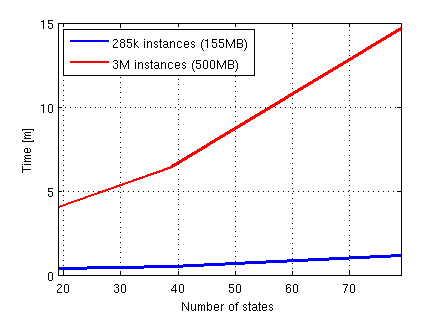
\includegraphics[width=0.7\columnwidth]{time-measurements}
	\caption{A graph of the measurements of the initial model construction time using two datasets, plotted against the number of states used for building the model. \lstopar{slabo napisano}}
	\label{fig:performance}
\end{figure}
We can see that although the construction time increases with the number of states, the initialization
procedure is quite fast for the smaller data set with only the larger model with 78 states taking over 
a minute to complete. \lstopar{When using the larger dataset ...}

\lstopar{
\begin{itemize}
	\item the larger dataset was constructed in acceptable time
\end{itemize}
}

\iffalse
\begin{tabular}{ c | c c c c c}
	\label{tab:time-tests}
	 & 10 & 20 & 40 & reading CSV & file size \\
	\hline
	3229541 & 11min & 13min 32s & 21min 50s & 6:58,7:05,7:10 & 500MB \\
	285168 & 1:31 & 1:36 & 2:17 & 1:09,1:06,1:08 & 155MB
\end{tabular}
\fi

\section{Experiments}
\label{sec:experiments}
\subsection{Prediction Evaluation}

This first experiment is intended to test the validity of our model. The model was constructed on simulated data of 
an electric motor and is shown in Figure \ref{fig:example-motor}. 
\begin{figure*}[]
  	\centering
  	\begin{subfigure}{.48\textwidth}
	  	\centering
	  	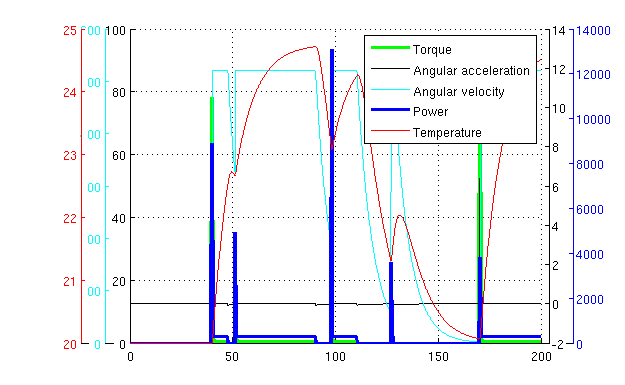
\includegraphics[width=\columnwidth]{simulation-processed}
  		\caption{\label{fig:simulation-chart}\lstopar{TODO}}
	\end{subfigure}
  	\begin{subfigure}{.48\textwidth}
	  	\centering
	  	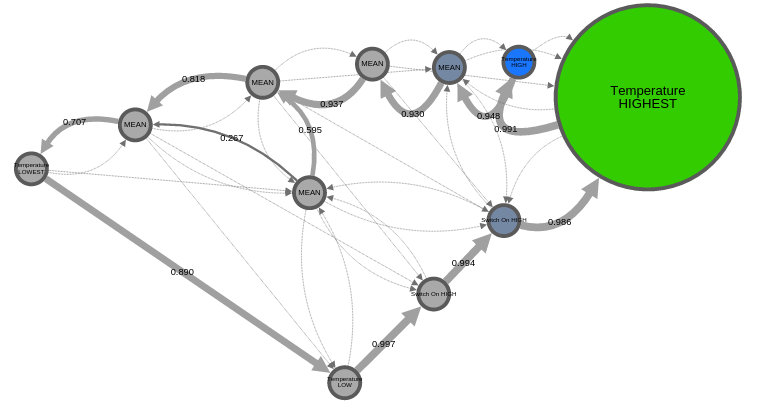
\includegraphics[width=\columnwidth]{model-motor-simulated}
  		\caption{\label{fig:simulation-model}\lstopar{TODO}}
	\end{subfigure}
  	\caption{\lstopar{TODO}}
  	\label{fig:example-motor}
\end{figure*}
The simulation starts in the leftmost state of Figure~\ref{fig:simulation-model} with the motor in a stationary state
and the power switch turned off. Then \lstopar{an invisible user} randomly, sampled from an exponential distribution,
toggles the "on" switch. Once the switch is on, as the rotation increases, the model starts moving in the counter clockwise
direction towards the large green state on the right. This state represents the \lstopar{equilibrium} when the temperature
gained through friction equals the temperature lost to the ambient and the \lstopar{signals} become \lstopar{stationary}.
Once the power switch is toggled again, the rotation slowly halts due to friction and the process goes from right to
left in the counter clockwise direction.

To conduct the experiment we generated two dataset: a training set and a test set. Both datasets
contained $200k$ observations. We built a StreamStory model with 20 lowest-level states on the training set using two attributes:
angular velocity and temperature. The training dataset was then replayed through the model and the finest scale states were stored. We then used
the stored states to calculate the transition probabilities and compared them to the models' jump chain $\Pi$. Since a lot of these probabilities were zero, we decided to use only the probabilities that
are non-zero either in the jump chain or in the probabilities calculated from the history. We then
computed the mean absolute error of the non-zero probabilities which resulted in $MAE=0.05$ or $5\%$.

In another experiment we tested the models predictive power. Two StreamStory models were built: (a) one 
model using the same attributes as in the first experiment, while in the second model (b), we used
the logical switch signal to model state transitions. The models were trained on the same dataset
as in the first experiment. Before the process jumped, we extracted the next state probabilities
and used the state with the highest probability as the predicted next state. We then computed
the prediction accuracy as the ratio between the number of correct predictions and the total number
of jumps (total number of predictions). In this experiment model (a) scored $0.845$ while model
(b) scored $0.904$.


\subsection{Weather Data}
\label{sec:experiments-weather}

The example below shows our model generated on monthly rainfall and temperature data
collected over the course of 20 years between 1920 and 1940 in Nottingham England.

\begin{figure}[h!]
	\centering
	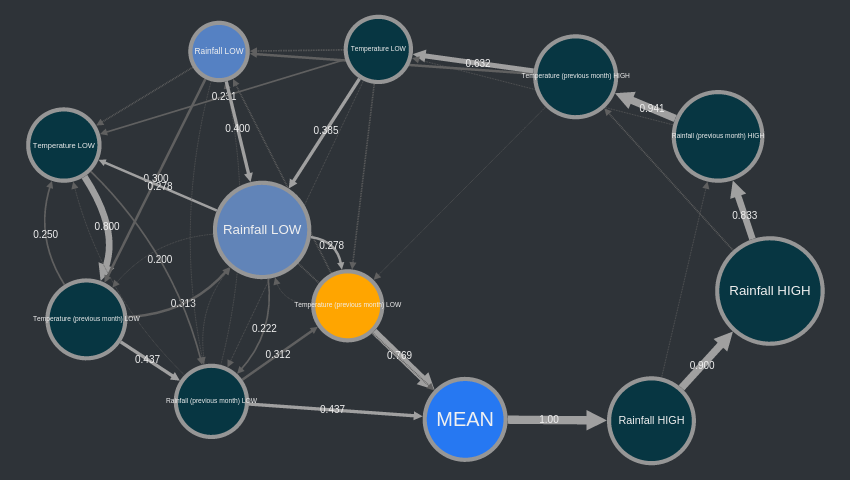
\includegraphics[width=\columnwidth]{example-weather}
	\caption{Qualitative representation of temperature and rainfall data collected over the course of 20 years.}
	\label{fig:example-weather}
\end{figure}

The model was generated using the raw rainfall and temperature data, but each feature vector includes
the rainfall and temperature of the previous month. The states on the right hand side represent the 
summer states, while the states on the left represent winter states. The yearly timeline flows in the
counter clockwise direction with the spring states residing on the bottom of the figure and the autumn
states on the top.

Interestingly, in this dataset, the rainfall and temperature are very highly correlated and the auto naming feature
choose high rainfall as the most significant feature of the summer states. This correlation can be seen
from the attribute histogram shown in Figure \ref{fig:histograms-summer}.

\begin{figure}[h!]
	\centering
	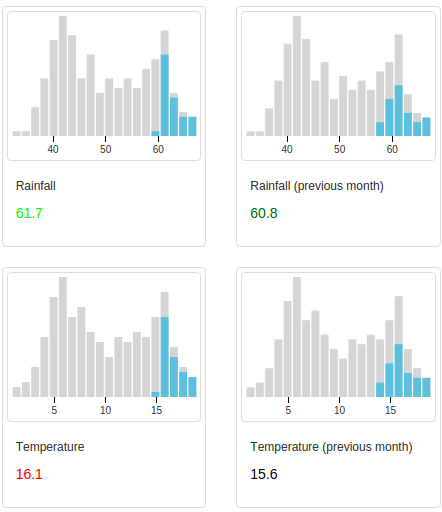
\includegraphics[width=0.5\columnwidth]{histograms-summer}
	\caption{\lstopar{TODO caption}}
	\label{fig:histograms-summer}
\end{figure}

\subsection{GPS Data}

The second example was created using raw GPS coordinates collected using a smartphone between \textcolor{red}{X} and \textcolor{red}{Y}.
The data represents the everyday movement of a European computer science researcher. Figure \ref{fig:example-geo}
shows our qualitative representation of this data on a high level with 8 state.

\begin{figure}[h!]
	\centering
	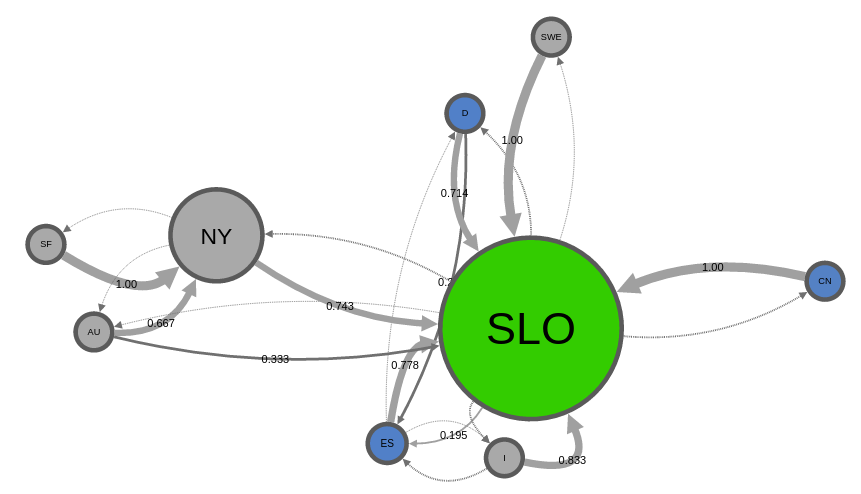
\includegraphics[width=\columnwidth]{geo-states}
	\caption{\lstopar{TODO caption}}
	\label{fig:example-geo}
\end{figure}

From the figure, we can see that the system was able to identify the most typical locations of this persons
movements. Most of the time they spend in central EU including two small states on the bottom and right
representing southern Europe and India where they went for vacation. On the European continent, the system
also identified Germany and Sweden where the person frequently attends meetings or stays for a short while
during a connecting flight. The states on the left represent the USA with the largest state representing New
York city where the person spent the 2014 summer and the smaller states representing San Francisco and Austin,
Texas.

\subsection{Traffic Data}

Our next example, shown in Figure \ref{fig:example-traffic}, shows a representation of a traffic counter positioned on the highway ring around Ljubljana.
\lstopar{In this example, we lifted the counter into a three dimensional space, by also including the number of
cars three hours and one day before.}
\begin{figure}[h!]
	\centering
	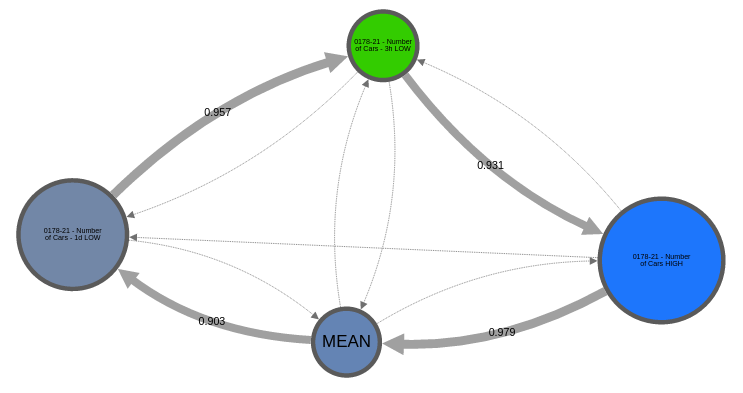
\includegraphics[width=\columnwidth]{example-traffic}
	\caption{\lstopar{TODO caption}}
	\label{fig:example-traffic}
\end{figure}
On a high level, our system was able to identify what we believe is the typical daily cycle on the highway ring.
The state on the left hand side represents a night state, when the traffic traffic is the lowest. This state
lasts from 10 PM to 5 AM when most people are asleep and not much is happening on the ring. Then, with a high 
probability, the system jumps into the topmost state with an above average traffic count which lasts from 6 AM
to roughly 9 AM. The next state is the midday state on the right with the highest traffic count lasting from 9 AM
to 7 PM. This is exactly the time when the traffic is very dense and most congestions occur. The next transition
is to the bottommost "evening" state with an average traffic count between 300 and 1000 cars per \lstopar{hour},
lasting from 8 PM to approximately 10 PM. 

\subsection{Domain Experts}

\section{Discussion}
\label{sec:discussion}


\begin{itemize}
	\item Kaj se zgodi, ce model updates v real time?
	\item Automatic description generation.
	\item theoretical guarantees
	\item  
\end{itemize}

%% if specified like this the section will be committed in review mode
\acknowledgments{
The authors wish to thank A, B, C. }

\bibliographystyle{abbrv}
%%use following if all content of bibtex file should be shown
%\nocite{*}
\bibliography{streamstory.bib}
\end{document}

